\documentclass[rep.tex]{subfiles}
\begin{document}

\chapter{Zadanie 13}
\label{zad13}
\section{Treść}
Zaprojektować czteroramienny, pierścieniowy sprzęgacz kierunkowy zapewniający przy
częstotliwości $f = 1.35~GHz$ sprzężenie $C = 3.01~dB$.
Sprzęgacz zrealizować z odcinków niesymetrycznej linii paskowej przyjmując,
że podłoże linii stanowi dielektryk o $\epsilon_r = 4.34$, $\mu_r = 1$ i grubości $h = 1.4~mm$.
Projekt wykonać przy założeniu, że grubość przewodu wewnętrznego $t = 0.035~mm$ a impedancja charakterystyczna linii obciążających sprzęgacz jest równa $Z_0 = 50~\Omega$.
Wyznaczyć częstotliwościową charakterystykę sprzężenia $C(f)~[dB]$ w paśmie od $f = 1.25~GHz$ do $f = 1.45~GHz$.

\begin{figure}[!htbp]
  \centering
  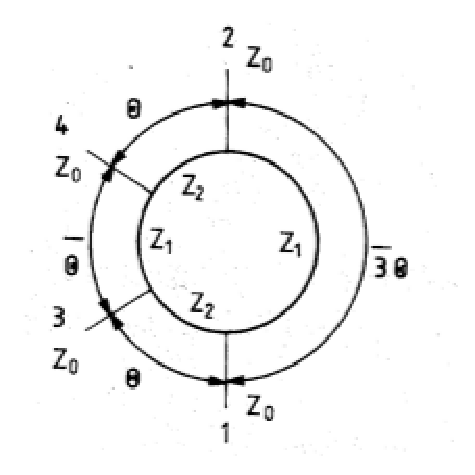
\includegraphics[width=0.5\linewidth]{fig/zad13/coupler_1}
  \caption{Schemat elektryczny sprzęgacza pierścieniowego}
  \label{fig:zad13:coupler1}
\end{figure}

\begin{figure}[!htbp]
  \centering
  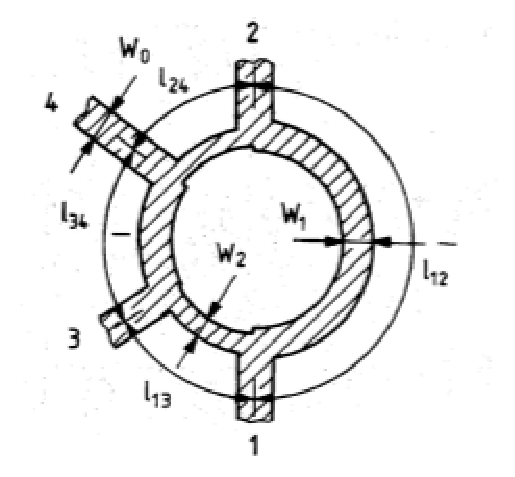
\includegraphics[width=0.5\linewidth]{fig/zad13/coupler_2}
  \caption{Realizacja sprzęgacza z niesymetrycznych linii paskowych}
  \label{fig:zad13:coupler2}
\end{figure}

\section{Rozwiązanie}
\subsection{Projekt sprzęgacza}
Rysunki~\ref{fig:zad13:coupler1} i~\ref{fig:zad13:coupler2} przedstawiają projektowany sprzęgacz.
Przy pobudzeniu wrót 4 wrota 2 i 3 są wyjściowe, synfazowe.
Sprzężenie pomiędzy wrotami $3$ i $4$ wynosi:
\begin{equation}
  C_{34} = 20 \log\Big( \frac{1}{|S_{34}|}\Big) = 10 \log\Big( \frac{1}{y_1^2}\Big) \label{eqn:zad13:C}
\end{equation}
gdzie:
\begin{align}
  y_1^2 + y_2^2 &= 1 \\
  y_1 &= \frac{Z_0}{Z_1} \\
  y_2 &= \frac{Z_0}{Z_2}
\end{align}
jest warunkiem na idealne dopasowanie impedancyjne wrót sprzęgacza.
Z równania~\ref{eqn:zad13:C} wynika zależność:
\begin{equation}
  y_1 = \sqrt{10^{-\frac{C_{34}}{10}}} = 0.707131200681
\end{equation}
Co pozwala wyznaczyć kolejne wielkości:
\begin{align}
  y_2 &= \sqrt{1 - y_1^2} &= 0.707082360848\\
  Z_1 &= \frac{Z_0}{y_1} &= 70.7082362535~\Omega \\
  Z_2 &= \frac{Z_0}{y_2} &= 70.7131202368~\Omega \\
\end{align}

Wyznaczone impedancje należy zamienić na odcinki niesymetrycznych linii paskowych tak samo jak było to wykonane w rozdziale~\ref{zad6}.
Szerokości ścieżek wynoszą:
\begin{align}
  w_1 &= 1.384465672~mm \nonumber \\
  w_2 &= 1.384261365~mm \nonumber
\end{align}

Podobnie jak w rozdziale~\ref{zad6} aby wyznaczyć długość odcinków ćwierćfalowych, należy obliczyć długość fali rozchodzącej się w linii.
Długość fali zależy od efektywnej przenikalności dielektrycznej~$\epsilon_{eff}$, która jest funkcją wymiarów oraz częstotliwości pracy.
Dlatego obliczono 2 różne długości.
Dla danych z treści zadania mamy:
\begin{align}
  \frac{\lambda_1}{4} &= 3.1315202668~cm \nonumber \\
  \frac{\lambda_2}{4} &= 3.13153691782~cm \nonumber
\end{align}

\subsection{Charakterystyka sprzęgacza}
W celu wyznaczenia charakterystyki częstotliwościowej wartości sprzężenie należy posłużyć się zależnością:
\begin{equation}
  C = 20 \log\Big(\frac{1}{|S_{34}|}\Big)
\end{equation}

\begin{align}
  S_{34} &= \frac{1}{2} \Big(S_{22}^{++} - S_{22}^{+-}\Big) \\
  S_{22}^{++} &= \frac{1 - A - B - jD}{1 + A + B + j(C + E)} \\
  S_{22}^{+-} &= \frac{1 - A' + B' - jD'}{1 + A' - B' - j(C' - E)} \\
\end{align}

Dokładne zależności podane zostały w~\cite{obwody}.
Charakterystykę sprzęgacza zaprezentowano na rys.~\ref{fig:zad13:freq}.

\begin{figure}[!htbp]
  \centering
  \includegraphics[scale=0.5]{fig/zad13/freq}
  \caption{Charakterystyka częstotliwościowa sprzęgacza}
  \label{fig:zad13:freq}
\end{figure}

\end{document}
